\documentclass[12pt,a4paper, hidelinks]{article}
\usepackage[utf8]{inputenc}
\usepackage{amsmath}
\usepackage{amsfonts}
\usepackage{amssymb}
\usepackage{amsthm}
\usepackage{graphicx}
\usepackage{hyperref}
\usepackage{geometry}
\geometry{a4paper, margin=1in}
\usepackage{fancyhdr}
\usepackage{indentfirst} % Add this line to enable first paragraph indentation
\usepackage{times} % Use Times New Roman font
\usepackage{setspace}
\usepackage{graphicx}
\usepackage{float}
\usepackage{listings}
\usepackage{tabularx}

\setstretch{1.15} % Adjust the stretch factor as needed

\pagestyle{fancy}
\fancyhf{}  % Clear header and footer fields
\rfoot{\thepage}  % Place page number at the right bottom corner
\renewcommand{\headrulewidth}{0pt}  % Remove the header line


\begin{document}

% Title Page
\begin{titlepage}
    \centering
    \vspace*{0.5 cm}
    
\includegraphics[width=0.20\textwidth]{images/logo.png}\par\vspace{1cm}
    {\scshape\LARGE Warsaw University of Technology \par}
    \vspace{1cm}
    {\scshape\Large Faculty of Mathematics and Information Science\par}
    \vspace{1.5cm}
    {\huge\bfseries Real-time fraudulent transactions detection \par}
    \vspace{1cm}
    {\Large\itshape Big Data Analytics\par}
    \vfill
    % \vspace{2cm}
    \begin{flushright}

    {\Large\textbf Salveen Singh Dutt (317298) \\ Karina Tiurina (335943) \\ Mikołaj Malec (298828) \\ Patryk Prusak (305794) \par}
    \vfill
    {Supervisor\par}
    {\Large mgr inz. Jakub Abelski \par}
    
    \end{flushright}
    \vfill
    % \break
    {\large Warsaw 2024\par}
    \vspace{1cm}
\end{titlepage}

\newpage

% Table of contents
\tableofcontents
\newpage % Optional: Add a page break after the TOC

\section*{Introduction}
\addcontentsline{toc}{section}{Introduction}

The goal of this project is to plan and implement financial transactions processing system which identifies suspicious and fraudulent activity in real-time. Given the large volume of incoming data, the project will utilize big data technologies as well as advanced machine learning algorithms for anomaly detection.

GitHub repository: \href{https://github.com/salveendutt/Big-Data-Analytics}{https://github.com/salveendutt/Big-Data-Analytics}.

\subsection*{Updates from Milestone 1}
\addcontentsline{toc}{subsection}{Updates from Milestone 1}
The project architecture layout was updated to better follow the Lambda architecture. In particular: 
\begin{itemize}
    \item master data storage was moved to the Batch layer;
    \item included NoSQL database as a storage for data querying in the Serving layer;
    \item Hive has been changed to Cassandra as the main storage solution;
    \item the architecture schema was updated to better represent the data flow. 
\end{itemize}


\section{High level description}

The main idea is to implement an automatic transactions processing so that anytime a fraudulent activity occurs, the transaction is blocked for further manual review. The aim is to reduce financial losses of the end-users and to enhance the security of online payment, ensuring a safer experience for all customers.

There are two main end-users of the project: financial institutions (we will call them 'Managers') and their customers executing the payments. Although both categories can benefit from the solution, in our implementation we will mainly focus on Managers to limit additional data in storage.

The list below contains main features that we expect to implement for Managers:
\begin{enumerate}
    \item Fraudulent transactions are automatically highlighted so that it is easier to identify suspicious activity;
    \item The history of transactions is stored and available for later review;
    \item A dashboard with statistics of fraudulent activity is available and customizable for better localisation of issues (e.g. too large amount, unusual location);
    \item Anomaly-detection model is continuously updated so that fraud detection utilizes new historical data and is more accurate on future transactions;
    \item Data streaming processing and batch jobs are customizable so that the testing of model's performance is simplified.
\end{enumerate}


\newpage

\section{Data sources}

Due to strict security regulations on personal and financial data, it is quite challenging to find open source real transactions data both for model training and streaming. Therefore, available synthetic and anonymized datasets will be used. The table below contains description of the data sources. Each data source is described in more detail in the dedicated subsections.

\begin{table}[h!]
\centering


\begin{tabular}{|p{4.8cm}|p{3.5cm}|p{2cm}|p{2cm}|p{1.5cm}|}
\hline
\textbf{Data Source} & \textbf{Content} & \textbf{Volume} &  \textbf{Fraud, \%} & \textbf{Link} \\
\hline
1. Fraudulent Transactions Data &  Dataset for predicting fraudulent transactions for a financial company. &  6,362,620 rows and 10 columns (493.53 MB) & 0.13\% & \href{https://www.kaggle.com/datasets/chitwanmanchanda/fraudulent-transactions-data}{Kaggle} \\
\hline
2. Credit Card Fraud & Contains features with transactional context. & 1,000,000 transactions (58.9 MB) & 8.7\% & \href{https://www.openml.org/search?type=data\&status=active\&id=45955}{OpenML} \\
\hline
3. Credit Card Transactions Synthetic Data Generation & A collection of synthetic credit card transaction data. & 1,785,308 transactions; 5,000 customers; (153.66 MB) & 3\% & \href{https://www.kaggle.com/datasets/cgrodrigues/credit-card-transactions-synthetic-data-generation?select=transactions_df.csv}{Kaggle} \\
\hline
4. Credit Card Fraud Detection & Transactions made by credit cards in September 2013 by European cardholders. & 284,807 transactions (150.83 MB) & 0.17\% & \href{https://www.kaggle.com/datasets/mlg-ulb/creditcardfraud}{Kaggle} \\
\hline
\end{tabular}

\caption{Data sources}
\end{table}

Data-streaming API was implemented from scratch. The assumption was that it would use the above datasets; with a specified time-frame, it would choose a random transaction which was not used for training and push it for further processing. For the testing purposes, the probability of a fraudulent transaction will be set manually to some high enough constant value. Details description of the implented streaming API can be found in chapter 3.

The content of the datasets is extremely different which makes it impossible to combine them into a single dataset. Therefore, each dataset will be treated separately for both streaming and ML training.


\subsection{Fraudulent Transactions Data (Kaggle)}

Dataset contains transactions for a financial company, indicating whether it is fraudulent or not. Data for the case is available in CSV format having 6362620 rows and 10 columns. Full column description is presented in the table 2.

\begin{table}[ht!]
\centering
\begin{tabular}{|p{3cm}|p{9.8cm}|p{2cm}|}
\hline
\textbf{Column} & \textbf{Content} & \textbf{Type} \\
\hline
step & maps a unit of time in the real world. In this case 1 step is 1 hour of time. Total steps 744 (30 days simulation) & int \\
\hline
type & type of the transaction. Available values: CASH-IN, CASH-OUT, DEBIT, PAYMENT and TRANSFER & str \\
\hline
amount & amount of the transaction in local currency & float \\
\hline
nameOrig & customer who started the transaction & str \\
\hline
oldbalanceOrg & initial balance before the transaction & float \\
\hline
newbalanceOrig & new balance after the transaction & float \\
\hline
nameDest & customer who is the recipient of the transaction & str \\
\hline
oldbalanceDest & initial balance recipient before the transaction. Note that there is not information for customers that start with M (Merchants) & float \\
\hline
newbalanceDest & new balance recipient after the transaction. Note that there is not information for customers that start with M (Merchants) & float \\
\hline
isFraud & this is the transactions made by the fraudulent agents inside the simulation. In this specific dataset the fraudulent behavior of the agents aims to profit by taking control or customers accounts and try to empty the funds by transferring to another account and then cashing out of the system & int \\
\hline
isFlaggedFraud & the business model aims to control massive transfers from one account to another and flags illegal attempts. An illegal attempt in this dataset is an attempt to transfer more than 200.000 in a single transaction & int \\
\hline
\end{tabular}
\caption{Columns description. Dataset 1: 'Fraudulent Transactions Data' from Kaggle}
\end{table}

The following transformation should be done to pass dataset to the ML models:
\begin{enumerate}
    \item 'type' column values CASH-IN, CASH-OUT, DEBIT, PAYMENT and TRANSFER transformed to 1, 2, 3, 4 and 5 respectively;
    \item a new attribute 'isMerchant' is calculated. 1 if 'nameDest' starts with 'M', 0 - otherwise.
\end{enumerate}

Generally, the dataset and clean and structured, no other preprocessing, except for the described above is necessary. Potential issue is that it is highly unbalanced (less than 1\% of fraud transactions), and contains quite small amount of features (6) for model training. 


\subsection{Credit Card Fraud (OpenML)}

This dataset captures transaction patterns and behaviors that could indicate potential fraud in card transactions. The data is composed of several features designed to reflect the transactional context such as geographical location, transaction medium, and spending behavior relative to the user's history.

\begin{table}[ht!]
    \centering
    \begin{tabular}{|p{5.5cm}|p{7cm}|p{2cm}|}
    \hline
    \textbf{Column} & \textbf{Content} & \textbf{Type} \\
    \hline
    distance\_from\_home & This is a numerical feature representing the geographical distance in kilometers between the transaction location and the cardholder's home address. & float \\
    \hline
    distance\_from\_last\_transaction & This numerical attribute measures the distance in kilometers from the location of the last transaction to the current transaction location. & float \\
    \hline
    ratio\_to\_median\_purchase\_price & A numeric ratio that compares the transaction's price to the median purchase price of the user's transaction history. & float \\
    \hline
    repeat\_retailer & A binary attribute where '1' signifies that the transaction was conducted at a retailer previously used by the cardholder, and '0' indicates a new retailer. & [0, 1] \\
    \hline
    used\_chip & This binary feature indicates whether the transaction was made using a chip (1) or not (0). & [0, 1] \\
    \hline
    used\_pin\_number &  Another binary feature, where '1' signifies the use of a PIN number for the transaction, and '0' shows no PIN number was used. & [0, 1] \\
    \hline
    online\_order & This attribute identifies whether the purchase was made online ('1') or offline ('0'). & [0, 1] \\
    \hline
    fraud & A binary target variable indicating whether the transaction was fraudulent ('1') or not ('0'). & [0, 1] \\
    \hline
    \end{tabular}
    \caption{Columns description. Dataset 2: 'Credit\_Card\_Fraud\_' from OpenML}
\end{table}

The whole dataset is in the numeric form, therefore, no additional preprocessing is necessary. The only transformation is to rename the target variable to 'isFraud' To match other datasets format.
The target feature balance is much better than for the previous dataset: 8.7\% of fraud. Additional complication is that feature 'amount' is not available. A ratio to the median purchase of the same customer is provided instead.


\subsection{Credit Card Transactions Synthetic Data Generation (Kaggle)}

This dataset is a collection of synthetic credit card transaction data. The data is designed to mimic the characteristics of real credit card transactions while ensuring privacy and compliance with data protection regulations such as the General Data Protection Regulation (GDPR). It contains 1,785,308 transactions for 5000 customers.

\begin{table}[ht!]
    \centering
    \begin{tabular}{|p{4.5cm}|p{8cm}|p{2cm}|}
    \hline
    \textbf{Column} & \textbf{Content} & \textbf{Type} \\
    \hline
    transaction\_id & Random string containing specific transactions id & str \\
    \hline
    post\_ts & Date and time of the transaction & str \\
    \hline
    customer\_id & Specific customer id & str \\
    \hline
    bin & Bank Identification Number & int \\
    \hline
    terminal\_id & Specific terminal id & int \\
    \hline
    amt & Transaction amount & float \\
    \hline
    entry\_mode & Mode of the transaction. Possible values are Contactless, Chip and Swipe. & str \\
    \hline 
    fraud & Target variable containing 1 for fraudulent transaction and 0 otherwise & int \\
    \hline
    fraud\_scenario & Additional label for the transaction. 97\% of the dataset has value 0. No specific description for each scenario is provided.  & int, [0, 1, 2] \\
    \hline
    mean\_amount & Average transaction amout for a specific customer  & float \\
    \hline
    std\_amount & Standard deviation of the transaction amout for a specific customer  & float \\
    \hline
    mean\_nb\_tx\_per\_day & Mean number of transactions per day for a specific customer & float \\
    \hline
    customer\_bin & Bank Identification Number of a customer & int \\
    \hline
    \end{tabular}
    \caption{Columns description. Dataset 3: 'Credit Card Transactions Synthetic Data Generation' from Kaggle}
\end{table}

Like other datasets, it is quite unbalanced with 3\% of fraudulent transactions. The following preprocessing should be done, before passing rows to ML task:
\begin{enumerate}
    \item 'entry\_mode' column values Contactless, Chip and Swipe transformed to 1, 2, and 3 respectively;
    \item 'amt' renamed to 'amount',
    \item 'fraud' renamed to 'isFraud',
    \item transaction data itself contains only customer id. Therefore, an additional step is to find the customer and add related features to the output.
\end{enumerate}


\subsection{Credit Card Fraud Detection (Kaggle)}

The dataset contains transactions made by credit cards in September 2013 by European cardholders. It contains 284,807 transactions with only 492 (less than 1\%) of fraud ones. Due to confidentiality issues, the dataset contains only numerical input variables which are the result of a PCA transformation.

\begin{table}[ht!]
    \centering
    \begin{tabular}{|p{2.5cm}|p{10cm}|p{2cm}|}
    \hline
    \textbf{Column} & \textbf{Content} & \textbf{Type} \\
    \hline
    Time & The seconds elapsed between the transaction and the first transaction in the dataset & int \\
    \hline
    V1 ... V28 & The principal components obtained with PCA. The original features and more background information about the data are not provided. & float \\
    \hline
    Amount & Transaction amount & float \\
    \hline
    Class & Target variable; 1 for fraudulent transaction and 0 otherwise & int, [0, 1] \\
    \hline
    \end{tabular}
    \caption{Columns description. Dataset 4: 'Credit Card Fraud Detection' from Kaggle}
\end{table}

This dataset contains relatively small amount of data compared to others (about 280k of transactions). Therefore, we are planning to keep it as an additional dataset in case of any issues with others.

Since the data has already been processed, the only necessary transormation is to rename columns 'Amount' and 'Class' to 'amount', 'isFraud' respectively.

\newpage

\section{Data acquisition strategy}

Due to the lack of publicly available open streaming APIs, we designed and implemented a custom streaming API for real-time fraud detection. Stream API is connected to the NiFi for futher data collection and preprocessing. The following technological stack is used for the data acquisition:

\begin{enumerate}
    \item Python,
    \item Flask  - for the stream API,
    \item Apache NiFi,
    \item Docker - for deployment,
    \item Apache Hive (to be properly configured for M3)
\end{enumerate}

When server is started, stream api is avalable on localhost:5000/data/:dataset\_id. Data frequency is configurable on the NiFi side and at the moment is set to 1 row per 10 seconds for each dataset. Format of each incoming transaction is JSON, containing attributes as described for each dataset in chapter 2. Example screenshots of the data stream and NiFi are provided in the SKaMP\_Tests.pdf file.

\section{Data storage strategy}

Our input data consists purely of a structured data and there is no need to store special data types, such as images, text files, audio and etc. Therefore, we diceded to utilize SQL-like data warehouse system that enables analytics at a massive scale - Apache Hive.

As described in chapter 2, our datasets contain completely different sets of features which makes it impossible to combine them in a single table. All incoming transactions will be divided into 4 groups for each dataset. Code block below represents an example of table creation for dataset 1 of the project.


\begin{lstlisting}[language=SQL, caption=Apache HIVE table creation]
    CREATE TABLE IF NOT EXISTS transactions_df_1 (
        step INT,
        type STRING,
        amount FLOAT,
        nameOrig STRING,
        oldbalanceOrg FLOAT,
        newbalanceOrig FLOAT,
        nameDest STRING,
        oldbalanceDest FLOAT,
        newbalanceDest FLOAT,
        isFraud INT,
        isFlaggedFraud INT
    )
    STORED AS TEXTFILE;
\end{lstlisting}

Preliminary list of all tables in the storage is the following:

\begin{enumerate}
    \item transactions\_d1 - raw data for the dataset 1;
    \item transactions\_processed\_d1 - processed data for the dataset 1;
    \item transactions\_d2 - raw data for the dataset 2;
    \item transactions\_processed\_d2 - processed data for the dataset 2;
    \item transactions\_d3 - raw data for the dataset 3;
    \item transactions\_processed\_d3 - processed data for the dataset 3;
    \item transactions\_d4 - raw data for the dataset 4;
    \item transactions\_processed\_d4 - processed data for the dataset 4.
\end{enumerate}

Additionally, we will be using MongoDB for storing prepared views for fast querying during the data presentation. Typically, it will replicate the processed data from both batch and streaming layers. This includes predicted labels for new transactions as well as indication whether data was used for training.


\section{Project architecture}

We are planning to implement the project based on Lambda Architecture. The main data processing will be divided into three layers:

\begin{enumerate}
    \item Speed Layer (streaming)
        \begin{itemize}
            \item Data preprocessing including transformation to a specific format;
            \item Real-time fraud detection on all of the incoming transactions.
        \end{itemize}
    \item Batch Layer
        \begin{itemize}
            \item Data processing and filtering for the model training
            \item ML model training with a fixed schedule (e.g. every 10 minutes)
        \end{itemize}
    \item Serving Layer
        \begin{itemize}
            \item Stores processed real-time and batch data in NoSQL for fast querying
            \item Client interface highlighting fraud transactions, accepting/blocking transactions;
            \item Data visualization with customizable filters
        \end{itemize}
\end{enumerate}

Figure 1 shows an outline of the project architecture.

\begin{figure}[htbp]
    \centering
    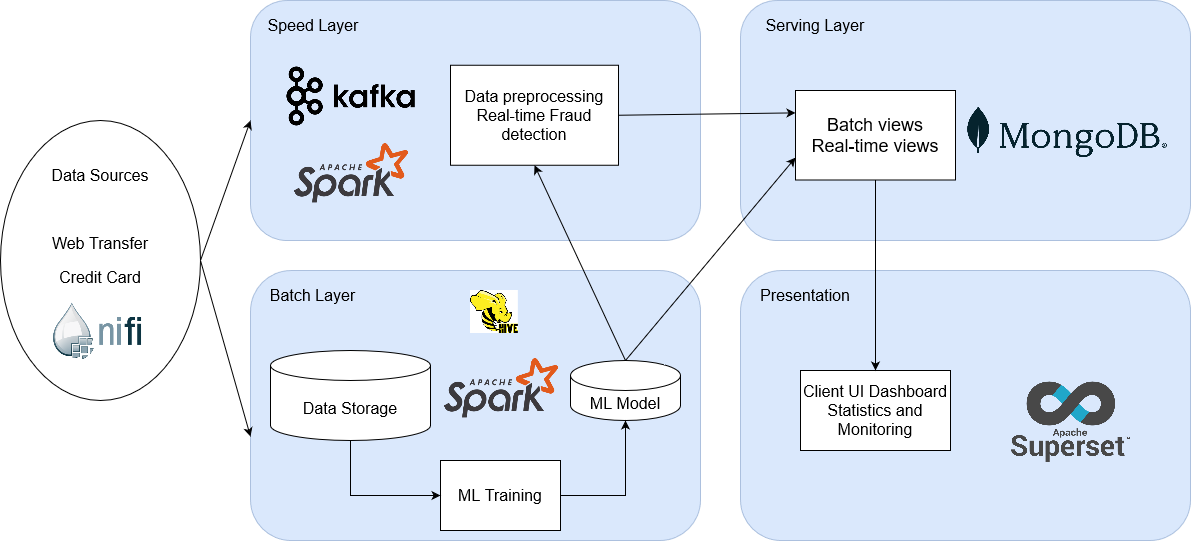
\includegraphics[width=0.95\textwidth]{images/Architecture-M2.png}
    \caption{Project architecture}
    \label{fig:sunset}
\end{figure}

The following Big Data platforms will be used:
\begin{itemize}
    \item Apache NiFi: to collect and distribute the data from different sources;
    \item Apache Hive as a data storage;
    \item Apache Kafka: to work with the streaming data;
    \item Apache Spark: to make the batch processing and model training;
    \item MongoDB: to store prepared batch view and real-time views for fast quering;
    \item Apache Superset (to be agreed with the supervisor): for data analysis on the user-interface. If the service will not be approved, UI will be implemented from scratch using JS framework, e.g. React.
\end{itemize}

\section{Planned ML Tasks}

This section explores potential machine learning tasks that could be applied to the available datasets for fraud and anomaly detection. The primary focus will be on identifying fraudulent transactions, developing anomaly detection models, and leveraging data-driven insights for effective fraud management. 

\subsection{Fraud Detection}
Fraud detection is a key use case for the provided datasets, where the goal is to classify transactions as fraudulent or legitimate. This can be achieved using various supervised learning techniques. Given that fraudulent transactions are typically rare, special care must be taken to handle the class imbalance. Planned steps include:
\begin{itemize}
    \item \textbf{Model Selection:} Applying binary classification models such as Logistic Regression, Random Forest, Gradient Boosted Trees (e.g., XGBoost, LightGBM), and Neural Networks. These models will be trained to predict the `isFraud` label in the datasets.
    \item \textbf{Evaluation Metrics:} Since fraud detection deals with imbalanced data, standard metrics such as accuracy are insufficient. Precision, recall, F1-score, and the area under the Precision-Recall curve (AUC-PR) will be used to evaluate model performance.
    \item \textbf{Imbalanced Data Handling:} Techniques such as SMOTE (Synthetic Minority Oversampling Technique), undersampling, or cost-sensitive learning will be explored to address class imbalance.
\end{itemize}

\subsection{Anomaly Detection}
Anomaly detection is a complementary task to supervised fraud detection, focusing on identifying unusual transactions that deviate significantly from normal behavior. This approach is particularly useful for uncovering previously unseen fraud patterns. Proposed methods include:
\begin{itemize}
    \item \textbf{Unsupervised Learning:} Techniques like Isolation Forests, k-means clustering, and DBSCAN will be applied to identify anomalous transactions based on transaction features. 
    \item \textbf{Autoencoders:} Neural network-based autoencoders will be used to reconstruct transaction data, with high reconstruction errors indicating potential anomalies.
    \item \textbf{Density Estimation:} Probabilistic models such as Gaussian Mixture Models (GMM) will be employed to estimate the likelihood of transactions and flag those with low likelihoods as anomalies.
    \item \textbf{Validation:} Anomalies detected by these methods will be cross-validated against the `isFraud` label to evaluate their effectiveness.
\end{itemize}

% \subsection{Customer Profiling and Behavioral Analysis}
% The synthetic dataset containing customer and terminal profiles provides an opportunity to perform behavioral analysis and create risk profiles. Proposed tasks include:
% \begin{itemize}
%     \item \textbf{Customer Segmentation:} Clustering techniques (e.g., k-means, hierarchical clustering) will be applied to group customers based on transaction behaviors, identifying high-risk segments.
%     \item \textbf{Terminal Risk Scoring:} Anomaly detection models will be used to identify terminals frequently involved in unusual or fraudulent transactions.
%     \item \textbf{Feature Engineering:} Time-based features (e.g., transaction frequency, average transaction amount over time) will be derived for deeper behavioral insights.
% \end{itemize}

\section{Planned batch and stream processing}

This chapter describes the planned implementation of batch and stream processing flows in detail, as part of the Lambda Architecture outlined in the previous section.

\subsection{Batch Processing Workflow}
Batch processing will focus on historical data analysis, feature engineering, and machine learning model training. The workflow for batch processing is as follows:

\begin{enumerate}
    \item Data Ingestion:
        \begin{itemize}
            \item Periodic ingestion of historical transactions from data storage sources (Apache Hive).
            \item Data preprocessing to validate and filter incomplete or invalid entries.
            \item Aggregation of transactional data for customer-level or terminal-level insights.
        \end{itemize}
    \item Data Transformation:
        \begin{itemize}
            \item Transformation of raw transaction data into structured formats suitable for ML model training.
            \item Feature engineering, such as creating rolling statistics (e.g., transaction frequency, average amount per customer, or terminal-specific patterns).
        \end{itemize}
    \item Model Training:
        \begin{itemize}
            \item Training ML models using the preprocessed data with a fixed schedule (e.g., every 30 minutes or daily, depending on model requirements).
            \item Storing the trained models in a model repository for use in the serving layer and the streaming layer.
        \end{itemize}
\end{enumerate}

\subsection{Stream Processing Workflow}
The stream processing layer will handle real-time fraud detection and serve as the system's speed layer. The workflow for stream processing is as follows:

\begin{enumerate}
    \item Data Ingestion:
        \begin{itemize}
            \item Continuous ingestion of live transaction data via Apache Kafka.
            \item Real-time preprocessing, including feature transformation (e.g., converting categorical variables, handling missing values).
        \end{itemize}
    \item Real-Time Fraud Detection:
        \begin{itemize}
            \item Use of trained ML models to perform predictions on incoming transactions.
            \item Updating fraud detection logic dynamically as new models are trained in the batch layer.
        \end{itemize}
    \item Event Streaming:
        \begin{itemize}
            \item Streaming results to MongoDB or another serving layer for downstream consumption.
            \item Flagging suspicious transactions for further analysis.
        \end{itemize}
\end{enumerate}

\subsection{Serving Layer Workflow}
The serving layer will provide a unified view of real-time and batch-processed data and offer tools for decision-making. The workflow is as follows:

\begin{enumerate}
    \item Unified Data Storage:
        \begin{itemize}
            \item MongoDB will serve as the primary storage for both batch and real-time data, enabling fast querying and retrieval.
        \end{itemize}
    \item Client Interfaces:
        \begin{itemize}
            \item Interfaces for visualizing flagged transactions in real-time.
            \item Fraud management tools to allow users to accept or block flagged transactions.
        \end{itemize}
    \item Data Visualization:
        \begin{itemize}
            \item Customizable dashboards for exploring transaction patterns, fraud rates, and model performance.
            \item Apache Superset will be evaluated as the primary visualization tool; if not approved, a custom solution will be implemented using React.
        \end{itemize}
\end{enumerate}

\subsection{Integration of Batch and Stream Processing}
The Lambda Architecture ensures seamless integration between the batch and stream processing layers:
\begin{itemize}
    \item ML models trained in the batch layer will be deployed to the stream processing layer for real-time fraud detection.
    \item Features engineered in the batch layer can inform the design of streaming features to ensure consistency.
    \item The serving layer will present a unified view of historical and real-time data, enabling holistic decision-making.
\end{itemize}

\section{Planned way of presenting the results}

In this architecture, we propose to use Apache Superset as the primary tool for presenting analytical results and monitoring system performance. Superset is an open-source data visualization and business intelligence platform that is well-suited for modern data pipelines due to its extensive support for a wide range of data sources and its ease of integration into existing architectures.

\subsection{Integration of Apache Superset with the Current Architecture}
As illustrated in the architecture diagram:
\begin{itemize}
    \item The \textbf{Batch Layer}, powered by Apache Hive, processes large-scale data and aggregates it into queryable formats. Superset can directly connect to Hive via SQL interfaces, enabling the creation of dashboards for historical and batch-processed data.
    \item The \textbf{Speed Layer}, which uses Kafka for real-time data ingestion and Spark for processing, produces real-time views that are stored in MongoDB. Superset can connect to MongoDB to display these real-time analytics, provided an appropriate SQL-like connector (e.g., MongoDB BI Connector) is configured.
    \item The \textbf{Serving Layer} facilitates the querying of both batch and real-time views, making this data accessible to Superset for visualization in unified dashboards.
\end{itemize}

By integrating Superset with both the batch and speed layers, the system can provide users with comprehensive dashboards that include both historical trends and real-time updates. This combination is particularly beneficial for monitoring critical use cases such as fraud detection, as it allows stakeholders to view both immediate alerts and long-term patterns.

\subsection{Advantages of Using Apache Superset}
\begin{itemize}
    \item \textbf{Ease of Use}: Superset provides an intuitive drag-and-drop interface for creating visualizations and dashboards, making it accessible to non-technical users.
    \item \textbf{Wide Data Source Support}: With native connectors for Hive and the ability to support MongoDB through connectors, Superset seamlessly integrates with the current architecture.
    \item \textbf{Real-Time and Batch Data Integration}: The ability to combine data from the speed and batch layers into unified dashboards enables comprehensive analytics and monitoring.
    \item \textbf{Custom Visualization}: Superset supports a variety of visualizations, allowing users to explore data in formats that best suit their needs, from basic bar charts to advanced geographic maps.
    \item \textbf{Scalability}: Being lightweight and web-based, Superset can handle a growing volume of data as the architecture scales.
    \item \textbf{Open Source and Extensibility}: As an open-source platform, Superset can be customized and extended to fit specific requirements.
\end{itemize}

\subsection{Disadvantages and Challenges}
While Superset provides significant benefits, there are a few challenges and limitations to consider:
\begin{itemize}
    \item \textbf{Indirect Support for Kafka}: Superset does not natively connect to Kafka. Real-time data from Kafka must first be stored in a queryable data store (e.g., MongoDB or a similar OLAP engine) before it can be visualized.
    \item \textbf{MongoDB Support}: Superset does not have native support for MongoDB. A SQL-like connector (such as the MongoDB BI Connector) or transformation of data into another supported format is required, adding some complexity.
    \item \textbf{Performance Considerations}: For real-time monitoring, performance can be a bottleneck if the underlying data stores (e.g., MongoDB or Hive) are not optimized for frequent querying by Superset.
    \item \textbf{Learning Curve for Advanced Features}: While the basic interface is user-friendly, advanced configurations (e.g., complex filters, custom SQL queries) may require technical expertise.
\end{itemize}


\section{Tasks assignment}

The table below contains the list of team members and preliminary allocation of tasks to team members.

\begin{table}[htbp]
\centering
\begin{tabular}{|p{4cm}|p{6.5cm}|p{4cm}|}
\hline
\textbf{Team member} & \textbf{Tasks} & \textbf{Supporter} \\
\hline
Salveen Singh Dutt & Batch processing of the historical data for up-to-date model training (Batch Layer). & Karina Tiurina \\
\hline
Karina Tiurina & Fraud detection model training and fine-tuning; Data stream processing (Speed Layer). & Salveen Singh Dutt \\
\hline
Mikołaj Malec & Data ingestion, collection and pre-processing. & Patryk Prusak  \\
\hline
Patryk Prusak & Data visualisation and configuration on the UI (Serving Layer). & Mikołaj Malec \\
\hline
\end{tabular}
\caption{Tasks assignment}
\end{table}

\newpage

\begin{thebibliography}{9}

    \bibitem{dataset1}
    Chitwan Manchanda,
    \textit{Fraudulent Transactions Data},
    Kaggle, 2022.
    Available at: \url{https://www.kaggle.com/datasets/chitwanmanchanda/fraudulent-transactions-data}.
    
    \bibitem{dataset2}
    \textit{Credit\_Card\_Fraud\_},
    OpenML, 2024.
    Available at: \url{https://www.openml.org/search?type=data&status=active&id=45955&sort=runs}.

    \bibitem{dataset3}
    Carlos José,
    \textit{Credit Card Transactions Synthetic Data Generation},
    Kaggle, 2024.
    Available at: \url{https://www.kaggle.com/datasets/cgrodrigues/credit-card-transactions-synthetic-data-generation?select=transactions_df.csv}.
    
    \bibitem{dataset4}
    Machine Learning Group - ULB and Andrea,
    \textit{Credit Card Fraud Detection},
    Kaggle, 2018.
    Available at: \url{https://www.kaggle.com/datasets/mlg-ulb/creditcardfraud}.
    

    \bibitem{dataset4}
    \textit{Lambda Architecture},
    Cazton.
    Available at: \url{https://cazton.com/consulting/enterprise/lambda-architecture}.

    \bibitem{chatgpt}
    OpenAI,
    \textit{ChatGPT: Language Model},
    Available at: \url{https://chatgpt.com}.
    
    \end{thebibliography}


\end{document}